\documentclass[tikz,border=2mm]{standalone}
\usepackage{pgfplots}
\pgfplotsset{compat=1.18}
\begin{document}
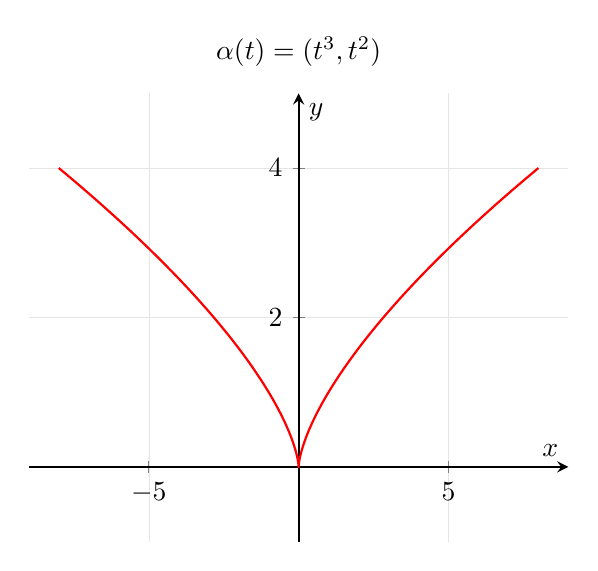
\begin{tikzpicture}
\begin{axis}[
    title={$\alpha(t)=(t^3, t^2)$},
    axis lines=middle,
    xlabel={$x$},
    ylabel={$y$},
    xmin=-9, xmax=9,
    ymin=-1, ymax=5,
    domain=-2:2,
    samples=100,
    grid=both,
    grid style={line width=.1pt, draw=gray!20},
    thick
]
\addplot[red, smooth, variable=\t] ({t^3}, {t^2});
\end{axis}
\end{tikzpicture}
\end{document}
